%%%%%%%%%%%%%%%%%%%%%%%%%%%%%%%
%This is the article LaTeX template for RSC journals
%Copyright The Royal Society of Chemistry 2010
%%%%%%%%%%%%%%%%%%%%%%%%%%%%%%%


\documentclass[8.5pt,twoside,twocolumn]{article}
\oddsidemargin -1.2cm
\evensidemargin -1.2cm
\textwidth 18cm
\headheight 1.0in
\topmargin -3.5cm
\textheight 22cm
\usepackage[super,sort&compress,comma]{natbib}
\usepackage{mhchem}
\usepackage{times,mathptmx}
% \usepackage{times}
% feel free not to use mathptmx if it causes difficulties
\usepackage{sectsty}
\usepackage{balance}

\usepackage{graphicx} %eps figures can be used instead
\usepackage{lastpage}
\usepackage[format=plain,justification=raggedright,singlelinecheck=false,font=small,labelfont=bf,labelsep=space]{caption}
\usepackage{fancyhdr}
\pagestyle{fancy}

\begin{document}

\thispagestyle{plain}
\fancypagestyle{plain}{
\fancyhead[L]{
\includegraphics[height=8pt]{headers/LH}}
\fancyhead[C]{\hspace{-1cm}
\includegraphics[height=20pt]{headers/CH}}
\fancyhead[R]{
\includegraphics[height=10pt]{headers/RH}\vspace{-0.2cm}}
\renewcommand{\headrulewidth}{1pt}}
\renewcommand{\thefootnote}{\fnsymbol{footnote}}
\renewcommand\footnoterule{\vspace*{1pt}%
\hrule width 3.4in height 0.4pt \vspace*{5pt}}
\setcounter{secnumdepth}{5}



\makeatletter
\def\subsubsection{\@startsection{subsubsection}{3}{10pt}{-1.25ex plus -1ex minus -.1ex}{0ex plus 0ex}{\normalsize\bf}}
\def\paragraph{\@startsection{paragraph}{4}{10pt}{-1.25ex plus -1ex minus -.1ex}{0ex plus 0ex}{\normalsize\textit}}
\renewcommand\@biblabel[1]{#1}
\renewcommand\@makefntext[1]%
{\noindent\makebox[0pt][r]{\@thefnmark\,}#1}
\makeatother
\renewcommand{\figurename}{\small{Fig.}~}
\sectionfont{\large}
\subsectionfont{\normalsize}

\fancyfoot{}
\fancyfoot[LO,RE]{\vspace{-7pt}
\includegraphics[height=9pt]{headers/LF}}
\fancyfoot[CO]{\vspace{-7.2pt}\hspace{12.2cm}
\includegraphics{headers/RF}}
\fancyfoot[CE]{\vspace{-7.5pt}\hspace{-13.5cm}
\includegraphics{headers/RF}}
\fancyfoot[RO]{\footnotesize{\sffamily{1--\pageref{LastPage} ~\textbar  \hspace{2pt}\thepage}}}
\fancyfoot[LE]{\footnotesize{\sffamily{\thepage~\textbar\hspace{3.45cm} 1--\pageref{LastPage}}}}
\fancyhead{}
\renewcommand{\headrulewidth}{1pt}
\renewcommand{\footrulewidth}{1pt}
\setlength{\arrayrulewidth}{1pt}
\setlength{\columnsep}{6.5mm}
\setlength\bibsep{1pt}

\twocolumn[
  \begin{@twocolumnfalse}
\noindent\LARGE{\textbf{The Spectral Networks Paradigm in High Throughput Mass Spectrometry}}
\vspace{0.6cm}

\noindent\large{\textbf{Adrian Guthals\textit{$^{a}$}, Jeramie D. Watrous\textit{$^{b,c}$}, Pieter C. Dorrestein\textit{$^{b,c}$} and
Nuno Bandeira\textit{$^{a,c,\ast}$}}}\vspace{0.5cm}
%Please note that \ast indicates the corresponding author(s) but no footnote text is required.

\noindent\textit{\small{\textbf{Received Xth XXXXXXXXXX 20XX, Accepted Xth XXXXXXXXX 20XX\newline
First published on the web Xth XXXXXXXXXX 200X}}}

%\noindent \textbf{\small{DOI: 10.1039/b000000x}}
\vspace{0.6cm}
%Please do not change this text.

\noindent \normalsize{High-throughput proteomics is made possible by a combination of modern mass spectrometry instruments capable of generating many millions of tandem mass (MS$^2$) spectra on a daily basis and the increasingly sophisticated associated software for their automated identification. Despite the growing accumulation of collections of identified spectra and the regular generation of MS$^2$ data from related peptides, the mainstream approach for peptide identification is still the nearly two decades old approach of matching one MS$^2$ spectrum at a time against a database of protein sequences. Moreover, database search tools overwhelmingly continue to require that users guess in advance a small set of 4-6 post-translational modifications that may be present in their data in order to avoid incurring substantial false positive and negative rates. The spectral networks paradigm for analysis of MS$^2$ spectra differs from the mainstream database search paradigm in three fundamental ways. First, spectral networks are based on matching spectra against other spectra instead of against protein sequences. Second, spectral networks find spectra from related peptides even before considering their possible identifications. Third, spectral networks determine consensus identifications from {\em sets} of spectra from related peptides instead of separately attempting to identify one spectrum at a time. Even though spectral networks algorithms are still in their infancy, they have already delivered the longest and most accurate {\em de novo} sequences to date, revealed a new route for the discovery of unexpected post-translational modifications and highly-modified peptides, enabled automated sequencing of cyclic non-ribosomal peptides with unknown amino acids and are now defining a novel approach for mapping the entire molecular output of biological systems that is suitable for analysis with tandem mass spectrometry. Here we review the current state of spectral networks algorithms and discuss possible future directions for automated interpretation of spectra from any class of molecules.
}
\vspace{0.5cm}
 \end{@twocolumnfalse}
  ]

\section{Introduction}

\footnotetext{\textit{$^{a}$~Dept. Computer Science and Engineering, University of California, San Diego; E-mail: bandeira@ucsd.edu}}
\footnotetext{\textit{$^{b}$~Department of Pharmacology and Department of Chemistry and Biochemistry, University of California, San Diego}}
\footnotetext{\textit{$^{c}$~Skaggs School of Pharmacy and Pharmaceutical Sciences, University of California, San Diego}}
\footnotetext{\textit{Published as part of a themed issue dedicated to Emerging Investigators}}

The success of tandem mass spectrometry (MS$^2$) approaches to peptide identification is partly due to advances
in computational techniques allowing for the reliable interpretation of MS$^2$ spectra. Mainstream computational techniques mainly fall into two categories: database search approaches that score each spectrum against peptides in a sequence database~\cite{eng94,perkins99,craig04,tanner05} and {\em de novo} techniques that directly reconstruct the peptide sequence from each spectrum~\cite{ma03,frank05,fischer05,mo07}. The combination of these methods with advances in high throughput MS$^2$ have promoted accelerated growth of spectral libraries - collections of peptide
MS$^2$ spectra whose identifications were validated by accepted statistical methods~\cite{keller02,elias07} and often also
manually confirmed by mass spectrometry experts. A similar concept of spectral archives was also recently
proposed to denote spectral libraries including "interesting" non-identified spectra~\cite{frank08} ({\em i.e.} unidentified recurring
spectra with good {\em de novo} reconstructions). The growing availability of these large
collections of MS$^2$ spectra has reignited the development of alternative peptide identification approaches
based on spectral matching~\cite{craig06,frewen06,lam07} and alignment~\cite{bandeira04,savitski06,bandeira07pnas} algorithms.

The dominant paradigm for high-throughput protein identification is based on trypsin digestion of extracted proteins to produce peptides followed by tandem mass spectrometry to generate single-peptide MS$^2$ spectra that are then computationally matched one spectrum at a time against protein sequence databases to finally obtain peptide and protein identifications. This paradigm has been the basis of nearly all large-scale proteomics studies to date despite its typical low spectrum identification rate of only 15-30\% because enzymatic digestion generates multiple peptides per protein and, in the extreme, only one peptide needs to be identified per protein (though more are usually preferred) to enable protein-level quantification and comparison across multiple tissues or experimental conditions. However, the serious downside of this low identification rate is that it consistently leads to missing information on non-tryptic peptides and yields very low protein sequence coverage, thus substantially limiting the chances of detecting alternative splicing or to identify and localize post-translational modifications (PTMs). In fact, the limitations of PTM search are so dire that most labs still only allow for 4-6 PTMs per search (about half or which due to sample handling procedures) even though more than 500 PTMs are known and listed in UniMOD.

Peptidomics, defined as the study of endogenous peptides, is an abundant source of drug candidates derived from neuropeptides~\cite{robertson11}, toxins~\cite{king11} and non-linear cyclic peptides~\cite{colgrave10}. Conversely, endogenous peptides are also valuable as therapeutic targets~\cite{jaggi11} (neuropeptides) and antigenic peptides are key in immunotherapeutic strategies~\cite{depontieu09} (MHC class-I/II peptides). Despite its critical importance, peptidomics research continues to suffer from the inadequate reutilization of computational tools primarily developed for proteomics since (a) endogenous peptides are not suitable for enzymatic digestion (as it eliminates the active peptide form), (b) tend to be modified with unexpected PTMs, (c) often contain sequence polymorphisms and (d) generally lack the "MS-friendly" features of trypsin-digested peptides. As such, each endogenous peptide must be identified "on its own" (not being able to benefit from multiple peptides per protein as in proteomics) and new identification algorithms are needed to be able to handle non-tryptic peptides of atypical lengths~\cite{jaggi11} (e.g., $\leq$6 AA or $\geq$35 AA) containing unexpected PTMs, sequence polymorphisms~\cite{klug09, colgrave10} and often featuring non-linear structures~\cite{king11,colgrave10}. Finally, Metaproteomics analysis of environmental samples from host-pathogen interactions~\cite{zheng11} and microbial communities (as in the Human Microbiome Project) requires the ability to search mass spectrometry data against very large databases and, in many cases, against six-frame translations of poorly-annotated genomes or even just assembled DNA reads. This enormous growth in the size of the sequences database and the need to allow for polymorphisms and/or unexpected PTMs results in a combined search space so large that 90-95\% of all spectra are commonly discarded as unidentified, thus severely limiting proteomics analysis of the role of microbiomes in health and disease~\cite{pflughoeft11}.

We argue that overcoming the identification bottleneck will require new ways of thinking about MS$^2$ spectra in order to develop new ways of interpreting them. In particular, we describe how the spectral networks paradigm differs from the current mainstream paradigm and illustrate its potential with applications where current paradigms perform poorly or completely fail. By finding spectra from related peptides even before considering their possible identifications and using these spectra to determine consensus identifications from sets of spectra from related peptides instead of separately attempting to identify one spectrum at a time, the spectral networking paradigm is capable of addressing many of the pitfalls of mainstream spectra identification paradigms. In addition to improving identification by significantly increasing signal-to-noise ratios and deconvoluting MS$^2$ ion types, spectral networks further open up new computational avenues for analysis of natural products and non-peptidic molecules, including compounds with non-linear structures, novel amino acids or post-translational modifications, lipids, glycans and other families of compounds.


\section{Spectral library matching}

The repeated acquisition and reliable identification of MS$^2$ spectra from a range of biological systems including various microbial species, mammalian tissues and cell lines has led to the accumulation of large collections of identified MS$^2$ spectra from mostly unmodified or partially modified peptide sequences. As a result, peptide identification by matching spectra of unidentified peptides against {\em spectral libraries} of identified peptide spectra~\cite{lam07} has recently gained new relevance, especially since the introduction of decoy spectral libraries~\cite{lam10} for calculation of false discovery rates~\cite{elias07,nesvizhskii10}. Searching against libraries of predicted spectra is also a promising emerging approach~\cite{yen09,yen11}.

The potential of spectral libraries to improve peptide identification is well illustrated by the recent example of the NeuroPedia~\cite{kim11neuropedia} spectral library of identified neuropeptide spectra. Neuropeptides are peptide neurotransmitters and hormones that mediate cell-to-cell communication for regulation of physiological functions and biological processes~\cite{hook10}. Understanding the role and regulation of neuropeptide forms in health, disease, and drug treatments requires the ability to globally analyze neuropeptide expression in an unbiased form. Mass spectrometry based neuropeptidomics is highly suited for untargeted, global neuropeptides studies~\cite{bora08,fricker07,hook10,li08,svensson07}. However, the unique characteristics  of neuropeptides ({\em i.e.} short/long sequences or non-tryptic) presents difficulties for identification from tandem mass spectrometry with traditional database search tools. For example, short neuropeptides can lead to inaccurate search results as database search tools usually assign lower scores to short peptides. Conversely, long or non-tryptic neuropeptides are difficult to identify since database search tools are trained for tryptic peptides cleaved at K/R and because peptide fragmentation processes for long neuropeptides is usually not efficient. In addition, as current databases mature, querying the larger search space requires more time due to the increase in the number of comparisons which ultimately reduces the number of identifications by allowing a higher probability for false positive matches~\cite{nesvizhskii10}. Since many spectral libraries, such as NeuroPedia, are directly searchable using mass spectrometry data, the caveats associated with matching experimental data against MS$^2$ spectra predicted from a protein sequence no longer apply as irregularities in fragmentation efficiency will be shared amongst the annotated and unannotated spectra. In addition to the expected improvement in sensitivity from searching against a small targeted sequence database, the neuropeptide spectral libraries further improve identification efficiency, sensitivity and reliability by considering all spectral features, including actual fragment intensities, neutral losses from fragments, and various uncommon or even unknown fragments to determine the best matches. As such, NeuroPedia was shown to improve peptide identification by up to ten fold (at the same false discovery rate~\cite{elias07,lam10,nesvizhskii10} but searching against a much smaller space of possible matches).

In addition to improving peptide identification, spectral library search opens up new possibilities for interpretation of MS$^2$ spectra. For example, mainstream approaches were developed under the ubiquitous assumption that each MS$^2$ spectrum is generated from a single peptide. While chromatographic procedures greatly contribute to making this a reasonable assumption, there are several situations where it is difficult or even impossible to separate pairs of peptides. Examples include certain permutations of the peptide sequence or post-translational modifications (PTMs, see~\cite{phanstiel08} for examples of co-eluting histone modification variants). In addition, innovative experimental setups have demonstrated the potential for increased throughput in peptide identification using mixture spectra - examples include Data-Independent Acquisition~\cite{venable04dia} Ion-Mobility Mass Spectrometry~\cite{masselon03} and MSE strategies~\cite{chakraborty07}. To address the resulting computational bottleneck, we introduced the first spectral library-based approach (M-SPLIT~\cite{wang10}) for identification of mixture spectra generated from more than one peptide. Theoretical bounds were proposed to prune the search space using branch-and-bound techniques and further improved using a new projected-cosine metric. In brief, M-SPLIT uses single-peptide matches to prune the search space for mixture peptides - it first matches experimental spectra to single-peptide spectra and then attempts to improve the score of the match by adding more single-peptide matches to form mixture-spectrum matches (false discovery rates also controlled using decoy spectral libraries~\cite{lam10}). Thus, M-SPLIT dramatically reduces the search space by six orders of magnitude and is able to deliver results at an average of 2 seconds/spectrum (on a regular laptop with a Pentium Core2Duo, 1.6Ghz, 2Gb RAM), even when searching against proteome-scale spectral libraries. Despite considering only a tiny fraction of the whole search space, benchmarks on both simulated and experimental data consistently show that M-SPLIT~\cite{wang10} has both high sensitivity ($\approx$94\%) and high accuracy (up to $\approx$98\%).

\section{Spectral networks of unidentified spectra}

The simplest example of a spectral network is the detection of MS$^2$ spectra from repeated acquisition of the same peptide in the same or multiple mass spectrometry runs; in these cases every node in the network is an individual spectrum in a separate run and edges between nodes indicate that the connected nodes represent spectra from the same peptide. Typically, in MS$^2$ analysis, each mass spectrum in the data set is searched against a sequence database. At times, this can be very inefficient since MS$^2$ data sets contain many redundancies (it is common for peptides to get selected for fragmentation more than once~\cite{tabb03a}). When mass spectra are collected from several runs, such redundancies can add up to hundreds and even thousands of spectra from the same
peptide. Instead of repeating the identification process for each spectrum, it can be beneficial to perform the search only once using a representative consensus spectrum per peptide and later apply the results to all similar spectra~\cite{tabb03a,beer04,tabb05}. By analyzing only representative spectra (one per cluster of spectra from each precursor mass), our MS-Cluster algorithm~\cite{frank08} scaled this approach for the analysis of tens of millions of spectra and resulted in a significant speed-up of MS$^2$ database searches (up to 10 fold) while simultaneously increasing the total number of identifications. Soon after, MS-Cluster was extended~\cite{frank11} to be able to process over $\approx$1.18 billion spectra acquired at Pacific Northwest National Lab over a period of 8 years. This extension served as the foundation for the proposed concept of {\em spectral archives}~\cite{frank11}, which extend spectral libraries by retaining both identified {\em and} unidentified spectra in the same way and maintaining information about peptide spectra that are common across species and conditions. Thus archives offer both traditional library spectrum similarity-based search capabilities along with new ways to analyze the data.

\subsection*{Spectral networks for analysis of post-translational modifications}

Samples of digested proteins often contain multiple overlapping peptides covering the same region of a protein sequence, such as prefix peptides (e.g. PEPTI/PEPTIDES), suffix peptides (e.g. TIDES/PEPTIDES) or partially-overlapping peptides (e.g. PEPTIDES/TIDESHIGH). In addition, most experimental protocols unintentionally generate multiple chemical modifications (e.g., oxidation) and it has been repeatedly shown that existing MS$^2$ datasets typically contain modified versions for many peptides~\cite{Hunyadi-Gulyas04, tanner05,tsur05,Wilmarth06}.
%
If the peptide sequences were known in advance, determining their overlap would be a straightforward application of the standard sequence alignment algorithms~\cite{smith81}. Conversely, spectral alignment is defined as the alignment of matching peaks between spectra from overlapping peptides~\cite{pevzner00,bandeira06}. This concept is illustrated in \mbox{Figure~\ref{figSpecNets}a} with the matching $b$-ions highlighted in blue. The surprising outcome of spectral alignment, as opposed to sequence alignment, is that even though one does not know the peptide sequences in advance, the sequence information encoded in the masses of the $b$/$y$-ions actually suffices to detect pairs of MS$^2$ spectra from overlapping peptides. In fact, it turns out that the reliability of spectral alignment allows one to discern the high-scoring true spectral pairs from the many millions of possible spectral pairs in high-throughput proteomics experiments~\cite{bandeira06,bandeira07pnas}. Moreover, since each spectrum may align to several other spectra, the set of detected spectral pairs defines a \emph{spectral network} where each node corresponds to a different spectrum and nodes are connected by an edge if the corresponding spectra were found to to be significantly aligned. This concept is illustrated in \mbox{Figure~\ref{figSpecNets}b-c} with spectral networks from human cataractous lens~\cite{bandeira07pnas} and a monoclonal antibody raised against the B- and T-cell lymphocyte attenuator molecule~\cite{bandeira08natbio}. Note that since most spectra usually come from non-contiguous protein regions, the consequent outcome of this approach is not a single spectral network but rather multiple spectral networks, one for each set of spectra from overlapping peptides.

In traditional DNA sequence alignment, it often happens that query sequences differ from the reference sequences by the insertion or deletion of one or more nucleotides~\cite{smith81}. While the insertion/deletion of amino acids is also usually allowed when aligning protein sequences, an additional factor needs to be considered when aligning peptides from experimental samples due to the occurrence of post-translational modifications. In fact, multiple groups have shown~\cite{tsur05,savitski06,na11} that the phenomenon of unexpected modifications is much more widespread
than commonly acknowledged.
%
From a sequence alignment perspective, a modification could be modeled by following the modified residue with a special character for each type of modification. Thus, the alignment of a modified peptide PEPT*IDE with its unmodified counterpart PEPTIDE would result in a single difference caused by the insertion of the modification `*'.
%
In tandem mass spectrometry, however, a modification of mass $m$ conceptually corresponds to the insertion of additional $m$~Da in the $b$/$y$-ion series between the ions immediately preceding and following the site of post-translational modification ({\em i.e.} the mass of the residue becomes larger by mass $m$). Conversely, if the modification causes a loss of $m$~Da from the modified residue then the corresponding effect is the subtraction of $m$~Da between the ions for the modified residue. When applied to unmodified and modified versions of the same peptide, the role of spectral alignment algorithms~\cite{pevzner01,bandeira04,bandeira07pnas} is to $a$) use the spectrum of the unmodified peptide to determine where to position the modification mass in the spectrum of the modified peptide and $b$) to assess whether the post-alignment match between the two spectra is significant enough to accept the spectra as a pair of modified/unmodified spectra from the same peptide. Thus, spectral alignment considers every possible spectral pair and every possible location for the mass difference ({\em i.e.} modification mass) between the aligned spectra. Figure~\ref{figSpecNets}a illustrates the spectral alignment between MS$^2$ spectra from the peptides TETMA and phosphorylated TET$^{+80}$MA. By requiring a significant match between the aligned spectrum peaks~\cite{bandeira07pnas} and by placing no restrictions on which modifications to consider, this approach can be used to discover novel or unexpected modifications. In fact, when applied to a set of spectra from cataractous lenses proteins from a 93-year old patient, spectral networks were able to rediscover the modifications identified by database search methods and additionally discovered several novel modification events~\cite{bandeira07pnas,tsur05}.

\begin{figure*}[!htb]
\centering
\scalebox{0.95}{\includegraphics{figures/figSpecNets.eps}}
\caption{Discovery and identification of post-translational modifications through spectral networks; \textbf{a)} Spectral alignment between modified and unmodified variants of the peptide TETMA ($b$-ions shown in blue, $y$-ions in red, blue/red lines track consecutively matched $b$/$y$-ions); \textbf{b)} Grouped modification states of the peptide MDVTIQHPWFK from a sample of cataractous lenses. Nodes in the spectral network represent individual MS$^2$ spectra and edges between nodes represent significant spectral alignments such as that shown in part (a); \textbf{c)} Spectra assembled in the spectral network for TNSMVTLGCLVK with diverse Cysteine modifications on a monoclonal antibody. Each arrow corresponds to the propagation of a sequence and/or PTM from an identified spectrum to an unidentified spectrum (repeated arrows are iterative propagations). Arrow colors correspond to types of modifications transferred.}
\label{figSpecNets}
\end{figure*}

When first analyzing a sample possibly containing modified peptides one does not know a priori which residues or peptides will be modified. Thus, spectral alignment considers every possible spectral pair and every possible location for the mass difference (e.g. modification mass) between the aligned spectra. By requiring a significant match between the aligned spectrum peaks~\cite{bandeira07pnas} but placing no restrictions on which modifications to consider, this approach can be used to discover novel or unexpected modifications. In fact, when applied to a set of spectra from cataractous lenses proteins from a 93-year old patient, spectral networks were able to rediscover the modifications identified by database search methods and additionally discovered several novel modification events~\cite{tsur05,bandeira07pnas} (~\ref{figSpecNets}).

The identification of peptides containing multiple modifications via database search is a challenging problem imparted by the combinatorial explosion in the number of possible modification variants for all the peptides in a database~\cite{tsur05,na11}. Not only can this make the approach much slower, but the increased number of peptide candidates for any given spectrum significantly increases the risk of incorrect identifications. However, samples containing peptides with two or more modifications often also contain variants of the same peptide with only one or no modification. In these cases, we have found that spectral alignment is able to group these related spectra from multiple modification variants of the same peptide into small spectral networks thus increasing confidence in their identity as a related peptide. Figure~\ref{figSpecNets}b illustrates the spectral network for a particular peptide in a sample of cataractous lenses proteins.

By grouping together spectra from multiple variants of the same peptide, spectral networks additionally contribute to the reliable identification of highly modified peptides. While database searching is restricted to matching ion masses between theoretical and observed spectra, spectral networks further capitalizes on the occurrence of common fragment ions at corresponding masses with similar peak intensities (Figure~\ref{figSpecNets}c). In general, it becomes easier to identify a highly modified peptide if one additionally observes highly-similar spectra from its intermediate modification states. Thus, spectral alignment not only allows one to \emph{discover} unexpected modifications (instead of only identifying expected modifications) but additionally provides an alternative route for identification of highly modified peptides.

\section{Shotgun Protein Sequencing}

Current approaches to proteomics focus on the reliable identification of proteins under the assumption that all proteins of interest are known and present in a database. However, the limited availability of sequenced genomes and multiple mechanisms of protein
variation often refute this assumption. Well known mechanisms of protein diversity include variable recombination and somatic hypermutation of immunoglobulin genes~\cite{gearhart02}. The vital importance of some of these novel proteins is directly reflected in the success of monoclonal antibody drugs such as Rituxan\texttrademark, Herceptin\texttrademark and Avastin\texttrademark~\cite{wiles06,haurum06,bandeira08}, of which all are derived from proteins that are not directly inscribed in any genome. Similarly, multiple commercial drugs have been developed from proteins obtained from species whose genomes are not known. In particular, peptides and proteins isolated from venom have provided essential clues for drug design~\cite{lewis03,pimenta05} - examples include drugs for controlling blood coagulation~\cite{joseph04,swenson04a,kini01} and therapeutic treatments for breast~\cite{swenson04,pal02} and ovarian~\cite{markland01} cancer. Despite this vital importance of novel proteins, the mainstream method for protein sequencing is still initiated by restrictive and low-throughput Edman degradation~\cite{ZugastiCruz06,ogawa04} - a task made difficult by protein purification procedures, post-translational modifications and blocked protein N-termini. These problems gain additional relevance when one considers the unusually high level of variability and post-translational modifications in venom proteins~\cite{buczek05,pimenta05a}.

Conceptually, sequencing a protein from a set of MS$^2$ spectra can be described by a simple analogy. Imagine a jewelry box with many identical copies of a specific model of bead necklaces. Although all the beads are identical, this model is characterized by having
irregular distances between consecutive beads \-- the set of inter-bead distances is initially chosen by the designer and all
necklaces are then made using exactly the same specification. Now assume that one day you open your jewelry  box and realize that
someone has vandalized all the necklaces by cutting them to fragments at randomly chosen bead positions. Can you recover the
original design of this model of necklaces, as specified by the set of consecutive inter-bead distances? In this allegory inter-bead distances correspond to amino acid masses and beads correspond to MS$^2$ fragmentation points (between consecutive amino acids). MS$^2$ data add more than a few difficulties to this necklace assembly problem; for example, most peaks in MS$^2$ spectra do not correspond to any fragment ions (extra beads) and many fragment ions do not result in any peaks (missing beads). Nevertheless, Figure~\ref{figSPS} presents an example of assembled MS$^2$ spectra resulting in a 22 amino acid long segment of a monoclonal antibody~\cite{bandeira08natbio}.

\begin{figure}[htb!]
\centering
  \includegraphics[height=15cm]{figures/figSPS.eps}
  \caption{Shotgun Protein Sequencing (SPS) via assembly of tandem mass spectra; \textbf{a)} Spectral alignment between spectra for peptide WSCILMEPKR (purple), PEWSCILMEPKR (green), WSCILMEPK (red), WSCILMoxEPK (cyan); Mox represents oxidized Methionine. Matching peaks in spectral alignments become pairwise gluing instructions between every pair of aligned spectra. \textbf{b)} Protein contig resulting from 24 spectra from a monoclonal antibody (aBTLA heavy chain). Each spectrum is shown superimposed with a sequence of arrows indicating its sequence of recovered masses; modified variants of the consensus sequence are indicated by red arrows (6 different modifications on 7 spectra). \textbf{c)} The complete aBTLA heavy chain sequence recovered by Comparative SPS~\cite{bandeira08}; highlighted sections were covered by protein contigs (95\% coverage) and the missing amino acids were obtained from homologous protein sequences.}
  \label{figSPS}
\end{figure}

Shotgun Protein Sequencing ({\em SPS}) is a {\em de novo} sequencing approach~\cite{bandeira04} that utilizes multiple MS$^2$ spectra from overlapping peptides generated using non-specific proteases or multiple proteases with different specificities~\cite{johnson87,klammer06,englander03,maccoss02a,pham06}. The original approach was based on the overlap~$\rightarrow$~layout~$\rightarrow$~consensus approach to assembly and shown to be efficient for the assembly of a single purified unmodified protein. However, practical applications (like sequencing snake venoms) require applicability to mixtures of modified proteins. In fact, most MS$^2$ samples contain both modified and unmodified versions for many peptides, including biological and chemical modifications both native and introduced during sample preparation. Sequence variations and post-translational modifications present a formidable algorithmic challenge for assembly algorithms as the performance of the original SPS approach~\cite{bandeira04} steeply degraded as soon as even a small percentage of the spectra are from modified peptides. To use the beads analogy, the necklace puzzle becomes very difficult if in addition to the canonical necklaces (non-modified proteins), the jewelry box also contains some necklaces that deviate from the designer's specification (modified proteins). Building on spectral networks algorithms for analysis of post-translational modifications based on alignment of spectra from modified and unmodified peptide variants~\cite{bandeira06,bandeira07pnas}, we showed how to integrate these alignments into Shotgun Protein Sequencing to derive a completely new form of spectral assembly. This utilized a generalized notion of {\em ABruijn~graphs} (originally proposed in the context of DNA fragment assembly~\cite{pevzner04}) for the assembly of MS$^2$ spectra from overlapping, modified and unmodified peptides into {\em contigs} (sets of aligned spectra from overlapping peptides, see Figure~\ref{figSPS}), where each contig then capitalizes on the corroborating evidence from the assembled spectra to yield a high-quality {\em consensus} {\em de novo} sequence. As a result, SPS consensus {\em de novo} sequences were found to be twice as accurate as sequences derived from single spectra (1 mistake per 10 vs 5 amino acid predictions) while yielding sequences that were much longer that single-peptide/spectrum could support (up to 24 AA long).

Recently this paradigm was extended in two distinct directions. First, we capitalized on homology between SPS long/accurate {\em de novo} sequences and known sequences to deliver the first automated full-length protein sequencing approach (Comparative SPS~\cite{bandeira08}) and demonstrated it with database-assisted {\em de novo} sequencing of two monoclonal antibodies. Spectral networks also underlie the related work of Castellana et al.~\cite{castellana10,castellana11}, who proposed an effective method for sequencing monoclonal antibodies with database-guided iterative alignment+assembly of spectra from overlapping peptides. Both of these methods rely upon the existence of a homologous database. To reduce this dependence, we have since developed MetaSPS~\cite{guthals12} algorithms for assembling SPS contigs into {\em meta-contigs} (sets of overlapping contigs). These methods now deliver {\em de novo} sequences over 100 AA long at sequencing error rates as low as 1 mistake per 50 predicted amino acids without requiring homology to known sequences, which demonstrates the feasibility of fully-automated {\em de novo} protein sequencing with unidentified MS$^2$ spectra. It is expected that the performance of these algorithms will only improve as new types of mass spectrometry data (e.g., Electron Transfer Dissociation) are also incorporated in SPS and spectral networks approaches.

\section{Spectral networks for non-ribosomal, cyclic peptides}

The central dogma of biology (translation of template mRNA into proteins/peptides) is not the only mechanism for cells to assemble amino acids into peptides. The alternative {\em Non Ribosomal Peptide Synthesis} is performed by a large multi-enzyme complex (called Non Ribosomal Peptide Synthetase or NRPS) that represents both the biosynthetic machinery and the mRNA-free template for the biosynthesis of secondary metabolites~\cite{sieber05,dorrestein06,welker06}. NRPS gene clusters produce relatively short (up to 50 AA) nonribosomal peptides (NRP) that are not directly inscribed in the genomic DNA and thus cannot be inferred with traditional DNA-based sequencing techniques. NRPs are of tremendous pharmacological importance since they were optimized during millions of years of evolution to play important roles in chemical defense and communication for producing organisms. Starting from penicillin, NRPs and other natural products ({\em i.e.} secondary metabolites) have an unparalleled track record in pharmacology: 9 out of the top 20 best-selling drugs were either inspired by or derived from natural products. NRPs have some naturally evolved features that are applicable to the modulation of protein function in human systems, making them excellent lead compounds for the development of novel pharmaceutical agents. In particular, NRPs include antibiotics (penicillin, cephalosporin, vancomycin, etc.), immunosuppressors (cyclosporine, tacrolimus, sirolimus), antiviral agents (luzopeptin A), antitumor agents (bleomycin), toxins (thaxtomin), and many peptides with yet unknown functions.

\begin{figure*}[!htb]
\centering
\scalebox{0.95}{\includegraphics{figures/figNRPs.eps}}
\caption{Analysis of the cyclic peptide Seglitide. \textbf{a)} The circular structure of Seglitide is schematically illustrated with each residue represented by a different color (slice sizes not scaled to corresponding masses of the residues). A$^{+14}$ denotes a non-standard residue with integer mass 71+14=85 Da. \textbf{b)} MS$^2$ fragmentation of Seglitide generates up to 6 linear peptides representing different rotated variants of the same cyclic peptide. \textbf{c)} Theoretical spectrum for Seglitide by superposition of the fragment masses of the linearized peptides. \textbf{d)} Experimental spectrum of Seglitide resulting from a mixture of 6 linear peptides (the peaks corresponding to fragment ions
are shown in red). \textbf{e)} Spectral network from assembled Seglitide MS$^n$ spectra and used for {\em de novo} sequencing with unknown amino acid masses.}
\label{figNRPs}
\end{figure*}

When DNA sequencing is not available, biologists use either Edman degradation or tandem mass spectrometry (MS$^2$) to sequence ribosomal peptides. However, neither of these approaches works for nonribosomal peptides since they differ from ribosomal peptides in many respects: (a) they often represent non-linear structures of amino acids (e.g., cyclic,  tree-like, and branch-cyclic peptides), (b) they often contain non-standard amino acids increasing the number of possible building blocks from 20 to several hundred, (c) they often have a non-standard backbone, and (d) they are often modified. Each of these complications renders traditional Edman degradation and MS$^2$ peptide sequencing approaches useless, leaving NMR as the only technology capable of analyzing NRPs~\cite{butcher06,williams05,luesch02,hamada05}. The use of NMR for NRP sequencing is time-consuming,
difficult to automate (there are currently no software tools for automatic interpretation of NRPs from NMR data), and  error-prone (see \cite{hamada05,ireland82} for examples of errors in NMR sequencing). In addition, the abundance of these specialized compounds {\em in vivo} is often very low requiring extensive raw biological material in order to purify enough of the compound to perform 2D NMR for structure elucidation. As a result, the extremely difficult process of total chemical synthesis remained one of the only reliable way to sequence and validate NRPs~\cite{Kurosawa05}.

Having shown how multi-stage mass spectrometry (MS$^n$) can improve {\em de novo} sequencing accuracy for linear peptides~\cite{bandeira08mann}, we then extended spectral networks algorithms using a combination of experimental and computational protocols to enable a mass-spectrometry based approach for {\em de novo} sequencing of cyclic peptides~\cite{bandeira08recomb}. The NRP-Sequencing algorithm discovers amino acid masses and reconstructs cyclic peptide sequences directly from a single MS$^3$ spectrum and MS$^4$/MS$^5$ spectra are used to rescore all putative MS$^3$ reconstructions. The NRP-Assembly approach assembles MS$^4$/MS$^5$ spectra, similarly to what was described above for Shotgun Protein Sequencing, and further integrates the resulting contig with the MS$^3$ spectrum and all non-assembled spectra (Figure~\ref{figNRPs}). These algorithmic foundations were further extended as more data became available~\cite{ng09} and we were able to show how these tools can conserve significant efforts using several marine cyanobacterial cyclic peptides. In particular, Cyanopeptide X was an unknown bioactive molecular whose identity was elucidated using the very time intensive workflow of isolating, purifying and collecting 2D NMR data to obtain the structure~\cite{liu09}. However, using very small amounts of raw material, sequencing of MS$^2$ data using our cyclic peptide annotation algorithms revealed that this compound was related to dolastatin 11 (reversed amino acid sequence with a single modification) and majusculamide C with identical scores, which provided great insight into the nature of the structure with very little time investment. The compound turned out to be desmethoxymajusculamide C and a full report on its structure as determined by NMR is now available~\cite{simmons09}. Another example was compound 879, which was initially assumed to be a novel compound but was later found to be already known during the patent application.  Our analysis could dereplicate the spectrum of compound 879 as the known NRP neoviridogrisen and could thus have saved the three years of effort it took to determine the structure.

\section{Spectral networks for any type of molecules}

Microbes use secreted factors to interact, communicate and manipulate their local environment and neighboring cell populations in a process known as metabolic exchange. By employing a wide breadth of molecules ranging from signaling compounds to defensive metabolites, metabolic exchange dictates not only basic microbial behavior such as biofilm formation, sporulation and motility, but also social interactions such as syntrophy and quorum sensing which enables microbes to establish communities~\cite{phelan11,ng09b,straight09,little08,lopez10,yim07,shank11,romero11}. Despite these secreted factors having a major impact on the phenotypic development of microbial populations, there is a lack of tools that enable scientists to probe the chemistry of microbial colonies in a direct manner, let alone of live microbial colonies. Currently the chemistry of microbes is studied indirectly and, in general, on single molecules -- an effort with a significant time and monetary investment.
%
Furthermore, since organisms are not static entities, it is important to be able to monitor chemical exchanges temporally and spatially as both the timing of production and the distribution of metabolic exchange factors within microbial populations can provide valuable insight into the function of these molecules.

\begin{figure}[htb!]
\centering
  \includegraphics[height=10cm]{figures/figMolSpecNets.eps}
  \caption{Molecular spectral network of a partial Bacillus subtilis secretome; nodes indicate MS$^2$ spectra of initially-unknown compounds of any class of molecules (no peptide-specific assumptions were made), and edges indicate significant similarity between the MS$^2$ fragmentation patterns of different spectra, mostly between intermediates/variants of the same compounds. Selected molecular structures are shown in black overlaid with the network and next to the correspondingly highlighted network clusters.}
  \label{figMolSpecNets}
\end{figure}

As with peptide-based spectral networks, molecular spectral networks~\cite{watrous12} start with raw MS$^2$ data acquired from one or more microbial species, irrespective of the number of spectra or mass spectrometry runs. Then, similarly to the algorithm illustrated in \mbox{Figure~\ref{figSpecNets}a)}, pairs of MS$^2$ spectra from related molecules are detected using {\em structure-independent} spectral alignment to find spectra with significantly-similar fragmentation patterns, regardless of whether the spectra are identified in advance or not. By avoiding peptide-specific fragmentation models and assumptions, structure-independent spectral alignment reveals molecular networks containing not only spectra of peptides but also primary and secondary metabolites, non-linear natural-products, lipids, glycans, and other classes of molecules. Figure~\ref{figMolSpecNets} shows a molecular spectral network for {\em Bacillus subtilis} 3610 and the chemical structures for several compounds corresponding to specific highlighted subcomponents of the whole network.

\section{Conclusions}

The spectral networks paradigm is founded on two core principles beyond mainstream approaches: $1)$ it is more efficient to match unidentified spectra to reference or other unidentified spectra than to reference sequences and $2)$ consensus interpretation of sets of related spectra is more reliable than identification of one spectrum at a time. In both instances it is relatively easy to see how these principles go beyond the potential of mainstream approaches. Reference spectra are also associated with reference sequences and annotations so additional knowledge of previously observed MS$^2$ fragmentation patterns can only improve identification algorithms. In addition to improving traditional peptide identification approaches, we have also shown how spectrum matching and library search algorithms~\cite{wang10} can support new directions such as identification of mixed spectra with more than one peptide beyond the state of the art in comparable database search approaches~\cite{wang10,wang11}. Also, having sets of spectra from related versions of the same compound (e.g., modified/unmodified, N/C-term extensions, CID/ETD/HCD/MS$^n$ spectra, etc.) significantly increases signal-to-noise ratios by providing more signal/fragmentation ions and averaging out inconsistent noise across all related spectra. As opposed to other multi-spectrum peptide identification and {\em de novo} sequencing approaches, spectral networks algorithms eliminate the need for the sets of spectra to be determined by the mass spectrometry instrument (e.g., as in MS$^2$/MS$^3$ protocols) and allow for correlation, alignment and assembly of spectra across multiple peptide sequence variations, post-translational modification, experimental conditions and even multiple species. The {\em de novo} sequencing subset of spectral networks algorithms (Shotgun Protein Sequencing, or SPS) clearly illustrates the potential of this approach by uniquely delivering {\em de novo} sequences longer than single-spectrum peptide sequences~\cite{bandeira07mcp} which now span over 100 amino acids at an average accuracy of less than one sequencing error per 50 AA~\cite{guthals12}. When combined with error-tolerant database search algorithms, SPS also enabled the first automated full-length protein sequencing approach, as demonstrated by our {\em de novo} sequencing of multiple monoclonal antibodies directly from a protein extract~\cite{bandeira08}.

As with spectral matching and library search, the potential of spectral networks algorithms extends beyond the scope of significantly improving on traditional uses of mass spectrometry data. Despite the significant clinical importance of natural products drug discovery, automated analysis of their mass spectra has always been tremendously challenging since these are often non-ribosomal and have no genomic propeptide template, are assembled with non-standard and heavily-modified amino acids and almost always have non-linear structures such as multi-cyclic, branched-cyclic and others - each of which renders traditional database search and {\em de novo} sequencing algorithms essentially useless. Using a combination of new mass spectrometry protocols and novel spectral networks algorithms, we showed~\cite{bandeira08recomb} how amino acid masses can be discovered directly from the data and how spectra of cyclic peptides can be assembled into accurate {\em de novo} sequences, a direction that was later explored for the analysis of several more novel natural products~\cite{liu09,ng09}. Building on these results and recent advances~\cite{watrous12}, the scope of spectral networks analysis has now been extended to the analysis of tandem mass spectra for any type of molecules by aligning spectrum fragmentation patterns without any prior assumptions on molecular structure or composition. As such, preliminary results indicate that the spectral networks paradigm may serve as the foundation to organize and search a mass spectrometry-centric view of the complete biomolecular space.

Being a relatively new paradigm~\cite{bandeira04,bandeira07pnas,bandeira07mcp}, the field of spectral networks analysis of tandem mass spectrometry data remains rich with open computational problems that stand to substantially benefit from additional developments in spectral matching, alignment, assembly and consensus interpretation. These and related developments continue to be proposed in closely related fields~\cite{wang10,yen11,lam11} and are expected to have a substantial impact on the quality and extent of future spectral networks repositories and tools.

\section*{Acknowledgements}

The Center for Computational Mass Spectrometry at UCSD is supported by the National Institutes of Health Grant 1-P41-RR024851 from the National Center for Research Resources. The P.C.D. laboratory is supported by US National Institutes of Health grants GM097509, GM094802, GM086283 and AI095125 and the Keck foundation.

\footnotesize{
\bibliography{../bibtex/msms,../bibtex/bandeiraLab,../bibtex/naturalproducts_venom,bibs/assembly,bibs/dna,bibs/theory,bibs/immunology}
\bibliographystyle{rsc} %the RSC's .bst file
}

\end{document}
